\section{Clustering}
\subsection{Supervised Learning}
\begin{itemize}
    \item Supervised Learning ist ein Ansatz des maschinellen Lernens, der sich durch die Verwendung von markierten Datensätzen auszeichnet
    \item Diese Datensätze dienen dazu, Algorithmen zu trainieren oder zu "überwachen", damit sie Daten klassifizieren oder Ergebnisse genau vorhersagen können
    \item Anhand der beschrifteten Eingaben und Ausgaben kann das Modell seine Genauigkeit messen und mit der Zeit lernen
    \item kann beim Data Mining in zwei Arten von Problemen unterteilt werden: \textit{Classification} und \textit{Regression}\\
\end{itemize}

\textbf{Classification}:
\begin{itemize}
    \item Bei Klassifizierungsproblemen wird ein Algorithmus verwendet, um Testdaten genau in bestimmte Kategorien einzuordnen, z.B. um Äpfel von Orangen zu unterscheiden
    \item In der realen Welt können Algorithmen des überwachten Lernens verwendet werden, um Spam in einen separaten Ordner Ihres Posteingangs zu klassifizieren
    \item Lineare Klassifizierer, Support Vector Machines, Entscheidungsbäume und Random Forest sind allesamt gängige Arten von Klassifizierungsalgorithmen\\
\end{itemize}

\textbf{Regression}:
\begin{itemize}
    \item weitere Methode des supervised Learnings, die einen Algorithmus verwendet, um die Beziehung zwischen abhängigen und unabhängigen Variablen zu verstehen
    \item Regressionsmodelle sind hilfreich für die Vorhersage numerischer Werte auf der Grundlage verschiedener Datenpunkte, wie z. B. Umsatzprognosen für ein bestimmtes Unternehmen
    \item \textit{beliebte Algorithmen}: lineare Regression, die logistische Regression und die polynomiale Regression
\end{itemize}

\subsection{Unsupervised Learning}
\begin{itemize}
    \item We are given Data (features, x) without labels (y) \textbf{=unlabeled data}, an we still learn something from the data?
    \item Yes! Often the data has some structure. \textbf{The goal} of unsupervised learning is to self-discover patterns from the data (find hidden patterns in the data)
    \item Data without any structure is the exception. But the structure can be hidden by noise.
    \item Humans are extremely efficient at noting patterns. But algorithms are extremely efficient at dealing with large and high-dimensional datasets where humans fail
\end{itemize}

\subsection{What is clustering?}
\begin{itemize}
    \item Group $n$ data points into $k_c$ number of clusters
    \item the data points within a cluster should behave similar
    \item Underlying assumption: similar data points are ''close'' together
    \item Similar = Data points which have shared properties (similar features)
\end{itemize}

\subsubsection{Applications}
\begin{itemize}
    \item Social Network Analysis
    \item Astronomical Data
    \item Marked segmentation
    \item Recommendation systems
\end{itemize}

\subsection{Naive K-means}
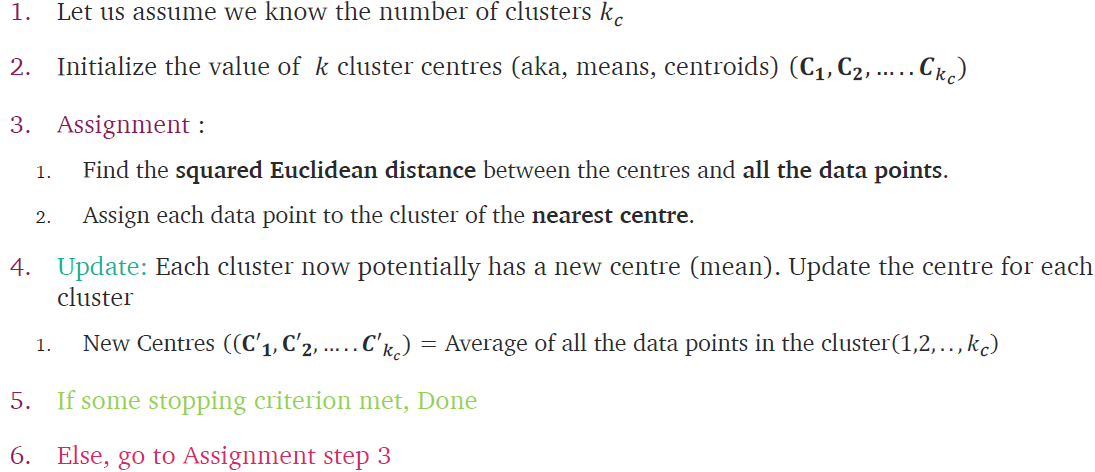
\includegraphics[width=\linewidth]{./img/k-means.png}
\subsection{K-Means Algorithm}
\begin{enumerate}
    \item Initially choose centers $C_1..C_{k_c}$ (can be random initialized)
    \item Assign step: Für alle Datenpunkte $j_1..N$ berechne die Distanz zu jeden Cluster-Center $C_1..C_{k_c}$. Dann jeder Datenpunkt dem Cluster zuordnen zu dem die Distance am geringsten ist
    \item Update step: Alle Center $C_1..C_{k_c}$ neu berechnen (mean of all data in cluster)
\end{enumerate}
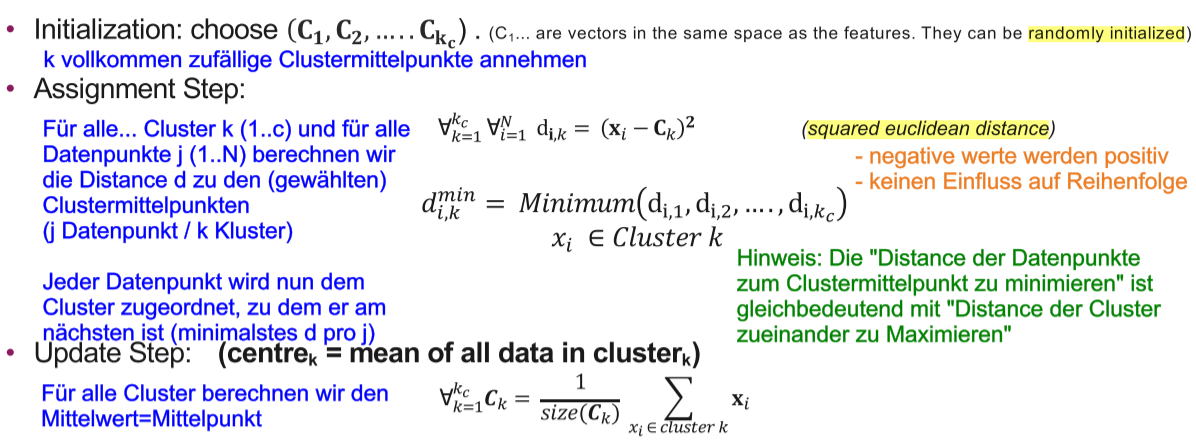
\includegraphics[width=\linewidth]{./img/w12_clustering_knn.png}

\subsubsection{Stopping Criterion}
\begin{itemize}
    \item When centres don't change (time consuming)
    \item The datapoints assigned to specific cluster remains the same (takes too much time)
    \item The distance of datapoints from their centres $>=$ treshold we have set
    \item Fixed number of iterations have reached (choose wisely)
\end{itemize}

\subsubsection{Initialization}
\begin{itemize}
    \item Performance depends on the random initialization
    \item Some seeds can result in a poor convergence rate
    \item Some seeds can converge to suboptimal clustering
    \item If centres are very close, it takes a lot of iterations to converge
    \item Initialize randomly, \textbf{run multiple times}
\end{itemize}

\subsubsection{Standardization of data (Scaling, Normalizing)}
\begin{itemize}
    \item Features with large values may dominate the distance value
    \item Features over small values will have no impact
    \item Normalize values! (Employ feature scaling with MinMaxScaler)
\end{itemize}
Verschiedene Skalierungen:
\begin{itemize}
    \item \textbf{Normalisierung} \python{MinMaxScaler}: Werte sind zwischen 0\dots1 (wichtig wenn Distanzen gerechnet werden)
    \item \textbf{Standardisieren} \python{StandardScaler}: Sodass Mittelwert=0 und Standardabweichung=1
    \item \textbf{Vector Normalisieren} \python{normalize}: Vector normalisieren auf Einheitsvektor (Länge $\sqrt{{x_1}^2 + {x_2}^2 + \dots}$ ergibt 1), macht das Rechnen einfacher resp. performanter
\end{itemize}

\subsection{Evaluation: Cluster Quality}
Choose the hyperparameter $k_c$ bigger than 1 and smaller than $N$. But what is a good values? Make clusters so that for each cluster the distance of each cluster member from its centre is minimized.

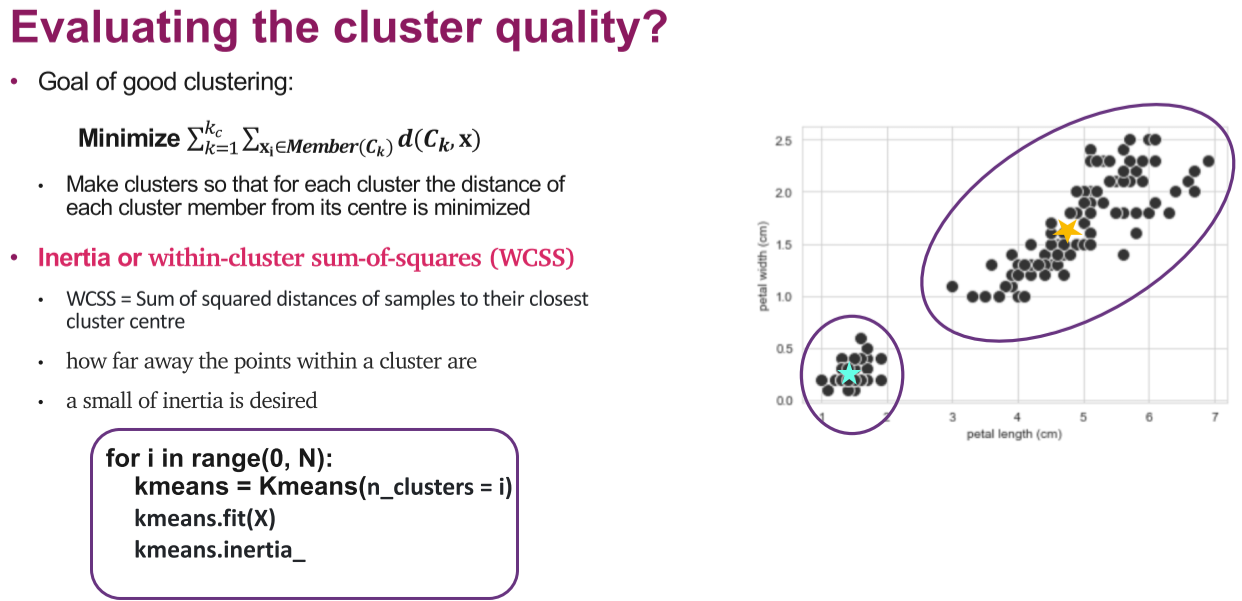
\includegraphics[width=\linewidth]{./img/w12_clusterquality.png}
\subsubsection{Inertia or within-cluster sum-of-squares (WCSS)}
\begin{itemize}
    \item Sum of squared distances to center
    \item ''Best'' cluster-size is where the ''elbow'' is (until sharp drop ends)
\end{itemize}
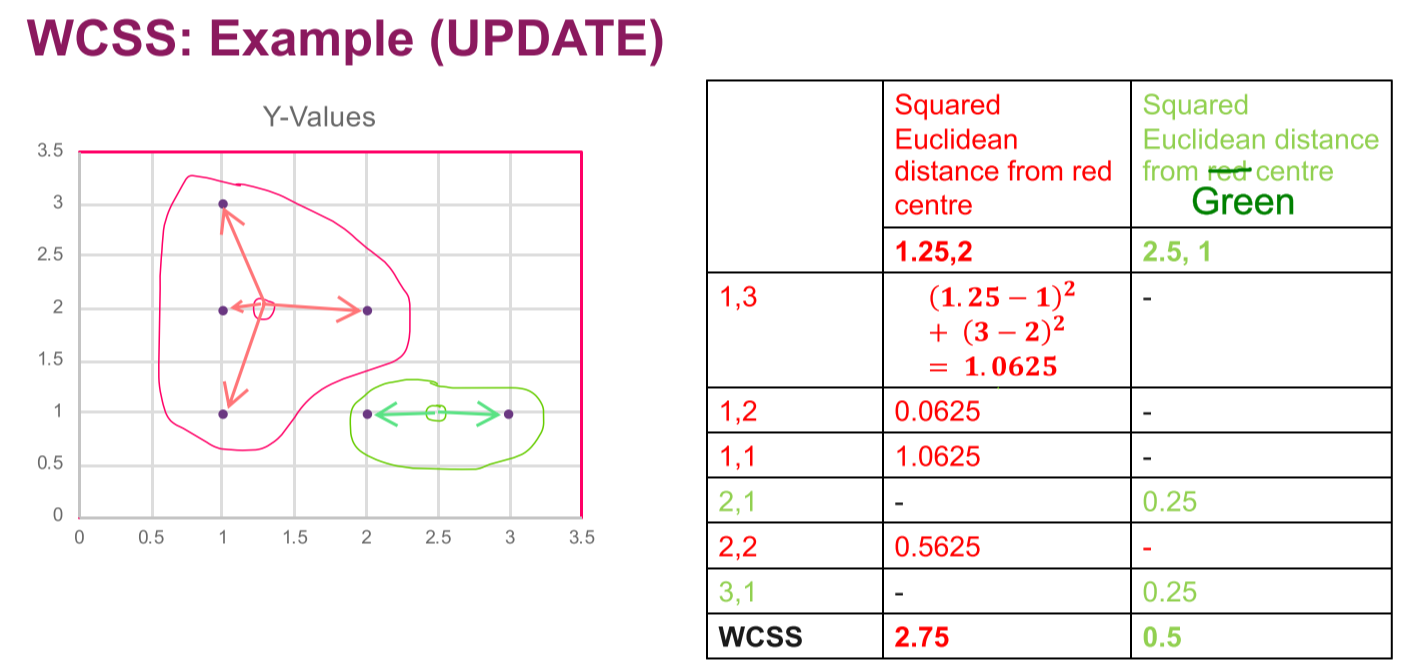
\includegraphics[width=\linewidth]{./img/w12_wcss.png}

\subsubsection{Silhouette Score}
\begin{itemize}
    \item \textbf{How far away the datapoints in one cluster are from the datapoints in another cluster}
    \item Silhouette Score of a point: $\frac{b-a}{max(a,b)}$
    \item $a$: average intra-cluster distance (distance between each point within)
    \item $b$: average inter-cluster distance (distance between a cluster and its nearest neighbour)
    \item Score should be close to 1 (good) and not close to -1 (bad)
    \item Silhouette Score of a cluster: mean of SS of each point in the cluster
\end{itemize}
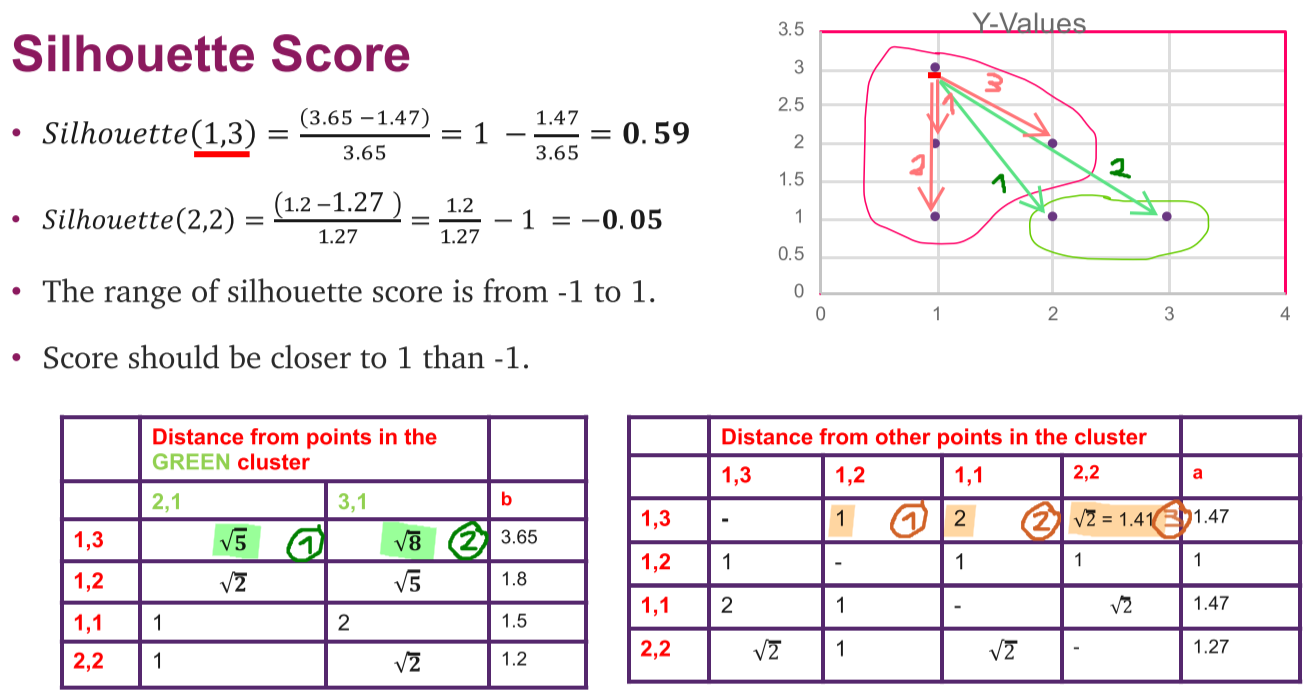
\includegraphics[width=\linewidth]{./img/w12_silhouette_score.png}

\subsubsection{How to choose number of clusters?}
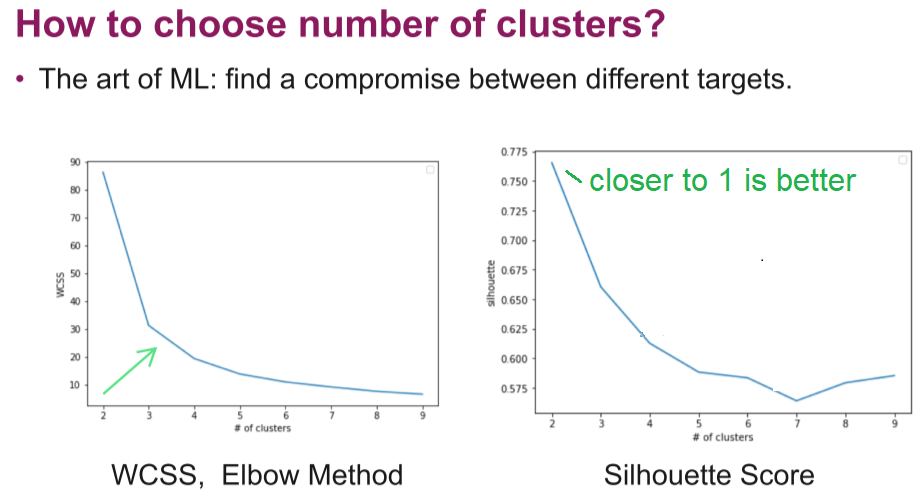
\includegraphics[width=\linewidth]{./img/w12_choose_nof_clusters.png}

\subsection{Implementation}
Aus sklearn-Folie: \python{from sklearn.preprocessing import MinMaxScaler} : data scaled wird aber in den Inclass-Notebooks niergends angewant (nur importiert)

\begin{minted}{python}
from sklearn.cluster import KMeans 
from sklearn.metrics import silhouette_score
from sklearn.preprocessing import normalize

#choose features
df = pd.DataFrame(iris.data, columns=iris.feature_names)
iris_3features = df.iloc[:, [0,1, 2]].values

kmeans = KMeans(n_clusters=2, init='k-means++', n_init=10, max_iter=300)
# - n_clusters = number of clusters (kc)
# - init = 'k-means++' selects initial cluster centers for k-mean clustering in a smart way to speed up convergence. 
# - max_iter = Number of iterations before stopping (stopping criterion)
# - n_init = Number of time the k-means algorithm will be run with different centroid seeds. 

# vector normalization
iris_3features= normalize(iris_3features)

# fitting the model to the data
kmeans.fit(iris_3features)

# output
print("cluster centres are", kmeans.cluster_centers_)
print("cluster labels of data points are", kmeans.labels_)
print ("Inertia is %f" %kmeans.inertia_)

# evaluate (different kc)
iterations = [], inertias = [], silhouettes = []
for k in range(kc_max):
  kmeans = KMeans(n_clusters=k)
  kmeans.fit(iris_3features)
  
  iterations.append(kmeans.n_iter_) #kmeans.n_iter_ is the number of iterations runs
  inertias.append(kmeans.inertia_)
  silhouettes.append(silhouette_score(iris_3features, preds))
\end{minted}